\documentclass[14pt]{matmex-diploma-custom}
\linespread{1.5}
\usepackage{listings}
\usepackage{cite}

\usepackage{tikz}
\usetikzlibrary{arrows}
\usepackage{amssymb}
\newcommand{\cd}[1]{\texttt{#1}}
\usepackage[caption=false]{subfig}
\usepackage{lstcoq}
\graphicspath{{images/}}%путь к рисункам

\lstdefinelanguage{haskell}{
keywords={data, type, case, of, where, otherwise, in, let, deriving},
sensitive=true,
basicstyle=\small,
commentstyle=\scriptsize\rmfamily,
keywordstyle=\ttfamily\underbar,
identifierstyle=\ttfamily,
basewidth={0.5em,0.5em},
columns=fixed,
fontadjust=true,
literate={->}{{$\to$}}1
}

\lstset{
basicstyle=\small,
identifierstyle=\ttfamily,
keywordstyle=\bfseries,
commentstyle=\scriptsize\rmfamily,
basewidth={0.5em,0.5em},
fontadjust=true,
escapechar=~,
language=haskell
}
%\DeclareMathSizes{16}{16}{16}{16}
\definecolor{dkviolet}{RGB}{100,0,100}
\definecolor{ltblue}{RGB}{0,100,100}
\definecolor{dkblue}{RGB}{0,50,50}

\begin{document}

\filltitle{ru}{
    chair              = {Кафедра Системного Программирования},
    title              = {История программных средств для доказательства теорем},
    author             = {ИЗМЕНИТЬ ИЗМЕНИТЬ ИЗМЕНИТЬ },
    supervisorPosition = {к.\,ф.-м.\,н.},
    supervisor         = {Кознов Д.\,В.},
}
\sloppy

%\maketitle
%\tableofcontents

\newpage
\section*{Введение}

\setlength{\unitlength}{1mm}
\begin{picture}(60, 40)
\put(20,30){\circle{1}}
\put(20,30){\circle{8}}
\put(20,30){\circle{16}}
\put(20,30){\circle{32}}

\put(25,10){\circle*{3}}
\put(30,10){\circle*{4}}
\put(35,10){\circle*{5}}
\put(0.3,4){$F=\sqrt{s(s-a)(s-b)(s-c)}$}
\put(2,3){\oval(13,5)}
\end{picture}
\newpage
\begin{center}


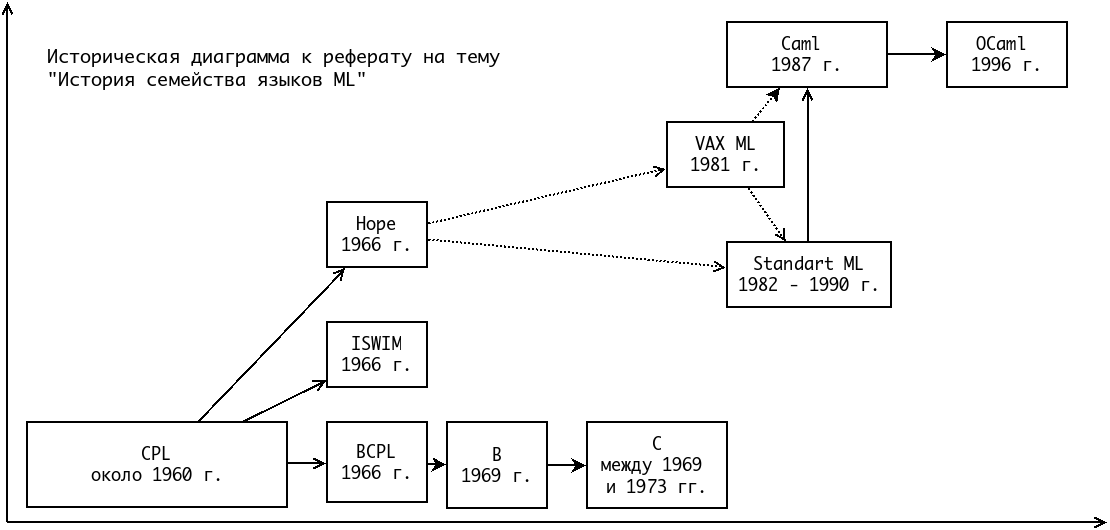
\includegraphics[angle=90,scale=0.585]{Diagram.png}
\end{center}

\newpage
\section{Возникновение теории типов}


\section{Теория типов Мартина-Лёфа}


\section{Исчисление конструкций Кокана}


\newpage
\section{Средства доказательства теорем}


\subsection{Coq}


\subsection{Agda}



\lstinputlisting{codes/a1.agda}


%\section{Сертификационное программирование}
\newpage
\section{Гомотопическая теория типов}


\newpage
\begin{thebibliography}{9}
  \bibitem{hilGeo}
    Д. Гильберт. Основания геометрии, перевод с немецкого под редакцией А.В.Васильева,
    Л., "Сеятель", 1923 — 152 с.
  \bibitem{kushner}
    Б.А. Кушнер. Лекции по конструктивному математическому анализу. — М.: Наука, 1973. — 447 с.
  \bibitem{taran}
    К. Таран. Метод применения Теории Типов Мартина-Лёфа для верификации программных систем.
    Дипломная работа, кафедра СП, СПбГУ, 2014.
  
  \bibitem{baren}
    H. Barendregt. Lambda Calculi with Types, Handbook of Logic in Computer Science, Volume II, Oxford University Press, 1991.
  \bibitem{coc}
    T. Coquand, G. Huet. The Calculus of Constructions, Information and Computation 76 (2–3), 1988.
  \bibitem{curry}
    H.B. Curry, R. Feys. Craig, William, ed., Combinatory Logic Vol. I, Amsterdam: North-Holland, 1958. p. 9E.
  \bibitem{gont}
    G. Georges. Formal Proof—The Four-Color Theorem, Notices of the American Mathematical Society 55 (11): 1382–1393, 2008.
  \bibitem{Hott}
    Homotopy Type Theory: Univalent Foundations of Mathematics. — Princeton: Institute for Advanced Study, 2013.
  \bibitem{howard}
    W.A. Howard. The formulae-as-types notion of construction, in Seldin, Jonathan P.; Hindley, J. Roger, To H.B. Curry: Essays on Combinatory Logic, Lambda Calculus and Formalism, Boston, MA: Academic Press, 1980 (original paper 1969). pp. 479–490
  \bibitem{makkai}
 M. Makkai. First Order Logic with Dependent Sorts, with Applications to Category Theory, 1995.
  \bibitem{progML}
    B. Nordström, K. Petersson, J. M. Smith. Programming in Martin-Löf's Type Theory. Oxford University Press, 1990.
  \bibitem{norell}
    U. Norell. Towards a practical programming language based on dependent type theory. PhD Thesis. Chalmers University of Technology, 2007.
  \bibitem{itt} P. Martin-Löf. Intuitionistic type theory,
    Studies in proof theory: Lecture notes (1), Giovanni Sambin, Bibliopolis, 1984.
  \bibitem{presburger}
    M. Presburger. Über die Vollständigkeit eines gewissen Systems der Arithmetik ganzer Zahlen, in welchem die Addition als einzige Operation hervortritt. Comptes Rendus du I congrès de Mathématiciens des Pays Slaves, 1929.  Warszawa. p. 92-101.
  \bibitem{russel1}
    A.N. Whitehead, B. Russell Principia mathematica 1 (1 ed.), Cambridge: Cambridge University Press, 1910.
  \bibitem{russel2}
    A.N. Whitehead, B. Russell. Principia mathematica 2 (1 ed.), Cambridge: Cambridge University Press, 1912.
  \bibitem{russel3}
    A.N. Whitehead, B. Russell. Principia mathematica 3 (1 ed.), Cambridge: Cambridge University Press, 1915.
  \bibitem{zhao}
     L. Zhaohui. Computation and reasoning: a type theory for computer science. Oxford University Press, Inc., 1994.
\end{thebibliography}

\end{document}
